\documentclass[12pt]{article}

\usepackage[utf8]{inputenc}
\usepackage[greek, english]{babel}
\usepackage{alphabeta}
\usepackage{libertine}
\usepackage{graphicx}
\usepackage{amsmath}
\usepackage[dvipsnames]{xcolor}



\title{3ο ΣΕΤ ΑΣΚΗΣΕΩΝ ΑΛΓΟΡΙΘΜΟΙ}
\author{\color{Mahogany}ΤΖΕΝΗ ΜΠΟΛΕΝΑ-3170117}
\date{}

\begin{document}

\maketitle

\section{\underline{Άσκηση 3.3}}
\subsection{Charts}
Χρησιμοποίησα Interpolation γαι την δημιουργεία του πολυωνίμου που εφαρμόζεται πάνω στα σημεία(μέθοδος LaGrange)! Χρήση Excel.
Τρέχοντας τα προγράμματα με διάφορα dataSet παρατηρουνται οι παρακάτω χρόνοι εκτέλεσης που εκφράζονται σε msecond:
 \begin{center}
	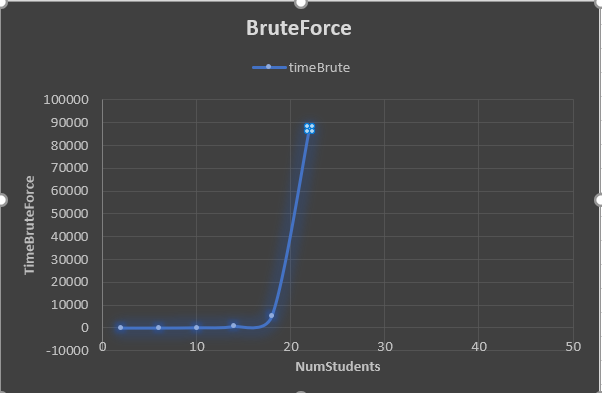
\includegraphics[scale = 0.7]{Brute.png}
\end{center}

 \begin{center}
	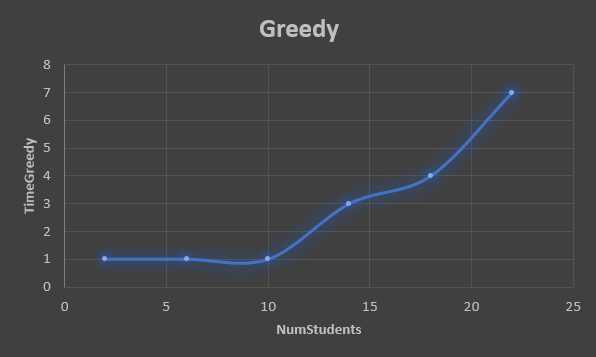
\includegraphics[scale = 0.7]{Greedy.png}
\end{center}

\subsection{Πολυπλοκότητα}
Το n αναφέρεται στο πλήθος των φοιτητών.
 \begin{itemize}
 	\item Greedy: $\mathcal{O}(n^3)$
 	\item BruteForce:$\mathcal{O}(2^n*n^2)$\\\\
 \end{itemize}

\subsection{Σχέση χρόνου εκτέλεσης-ποιότητας αποτελέσματος}
Παρατηρούμε ότι ο greedy τρέχει πολύ πιο γρήγορα απο τον bruteForce ειδικά όσο το πλήθος των φοιτητών αυξάνεται. Ωστόσο ο greedy δεν δίνει πάντα το βέλτιστο αποτέλεσμα, ενώ με τον brute force το αποτέλσμα είναι πάντα βέλτιστο!\\
Παρακάτω δίνεται παράδειγμα που ο greedy δεν δίνει βέλτιστο αποτέλεσμα.

 \begin{center}
	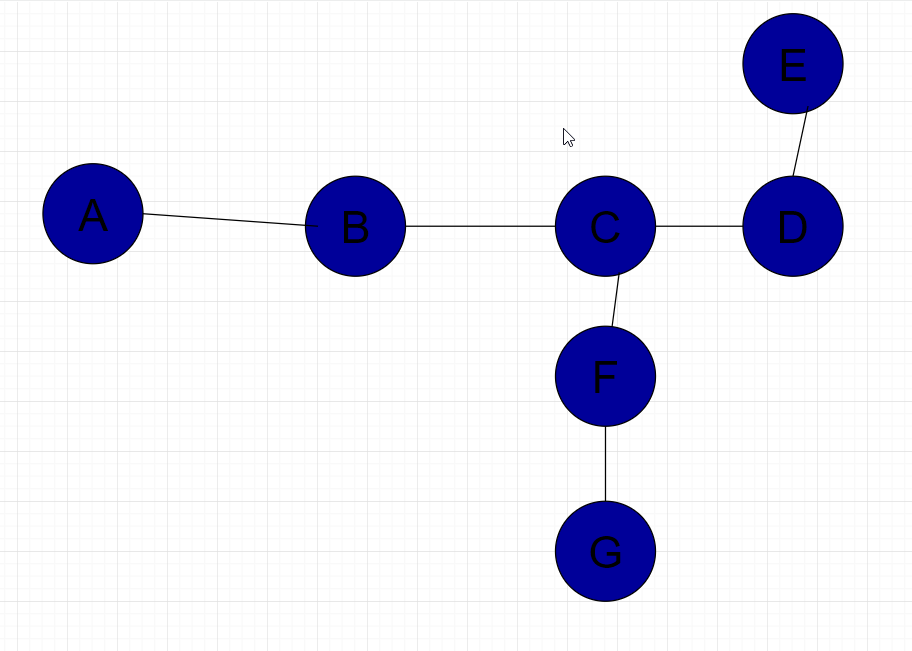
\includegraphics[scale = 0.7]{GreedyNotBestSolution.png}
\end{center}
Στην παραπάνω εικόνα που έφτιαξα μέσω του drawIO, o Greedy έχει σαν λυση τα vertices {C, A, E, G}, ενώ ο BruteForce έχει βέλτιστη λύση {B, D, F}. Επομένως αν και ο greedy κερδίσει σε ταχύτητα χάνει σε ποιότητα. \\\\


\section{\underline{Άσκηση 3.4}}
Το πρόβλημα Dominating Set είναι $NP$, αρκεί να αποδείξουμε ότι υπάρχει ένα $NP-Complete$ πρόβλημα που ανάγεται σαυτό και θα καταλήξουμε στο ότι είναι $NP-Complete$!\\
Θα κάνουμε την εξής αναγωγή(reduction): $Vertex Cover\le_P Dominating Set$\\\\
(Θέλω να δείξω ότι $\mathcal{G}$ έχει Vertex Cover αν και μόνο ανν $\mathcal{G'}$ έχει dominating Set)\\
Δεδομένου ενός γράφου $\mathcal{G} = (V,E)$ και ενός $k$ που δηλώνει ένα τόσο μεγάλο Vertex Cover, μετατρέπουμε αυτό σε στιγμιότυπο του Dominating Set. Όπως είδαμε και στο μάθημα μπορούμε να πάρουμε  ένα στιγμιότυπο $I$ του Vertex Cover  και μέσω μιας συνάρτησης μετασχηματισμού $f$ να έχουμε πλέον ενα στιγμιότυπο $f(I)$ του Dominating Set. Aπο τον γράφο $\mathcal{G}$ μπορούμε να φτιάξουμε ενα νέο γράφο  $\mathcal{G'} = (V',E')$ ο οποίος για κάθε ακμή $(u,v)$ του  $\mathcal{G}$ θα προσθέτει εναν νέο κόμβο(vertice) $t$ ο οποίος θα έχει ακμή με τους κόμβους $u, v$. \\

  Είναι προφανές ότι ενα Vertex Cover του $\mathcal{G}$ είναι Dominating Set του $\mathcal{G'}$, αυτό μπορούμε να το κατλάβουμε ευκολά αν σκεφτούμε το minimum Vertex Cover ενός δυαδικού δέντρου.//
  Για να δείξουμε τώρα ότι ένα dominating set του $\mathcal{G'}$ είναι και vertex cover του $\mathcal{G}$ λέμε το εξής: Αν $DS$ το dominating set του $\mathcal{G'}$ τότε αν αυτό περιέχει μία από τις νέες ακμες(αυτές δλδ που δεν υπάρχουν στον $\mathcal{G}$) αυτές επειδή συνδέονται η κάθε μια μόνο με δύο κόμβους που έχουν ακμή μεταξύ τους, μπορούμε να τις αγνοήσουμε και έτσι έχουμε ακόμη  dominating set. Απο αυτό γίνεται κατανοητό ότι το $DS$ περιέχει μόνο κόμβους από τον $\mathcal{G}$. Και το $DS$ είναι και vertex cover του $\mathcal{G}$ επειδή για κάθε ακμή $(u,v)$  πρέπει ένας απο τους δύο κόμβους να ανήκει στο dominating set έτσι ώστε να καλύπτεται και ο νέος κόμβος που προσθέσαμε( ο κόμβος $t$).\\
  Επομένως καταλήγουμε στο συμπέρασμα ότι ο $\mathcal{G}$ έχει vertex cover μεγέθους $κ$ αν και μόνο αν o $\mathcal{G'}$ έχει dominating set μεγέθους $κ$.
  
  \textbf{Αρα το πρόβλημα Dominating Set είναι NP-Complete!}
  



\end{document}
